\begin{figure}
%\makebox[\textwidth]{\framebox[10cm]{\rule{0pt}{250pt}}}
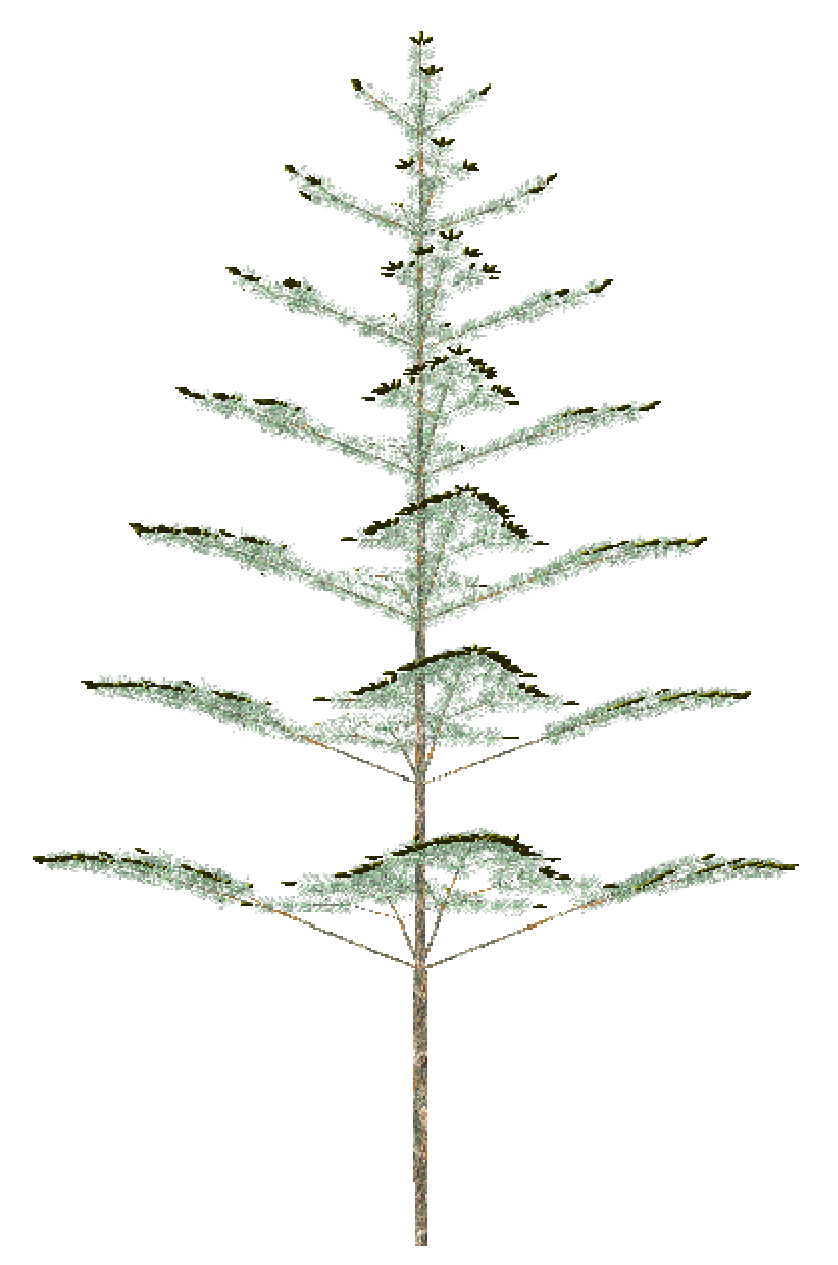
\includegraphics[scale=0.25]{pineL8}
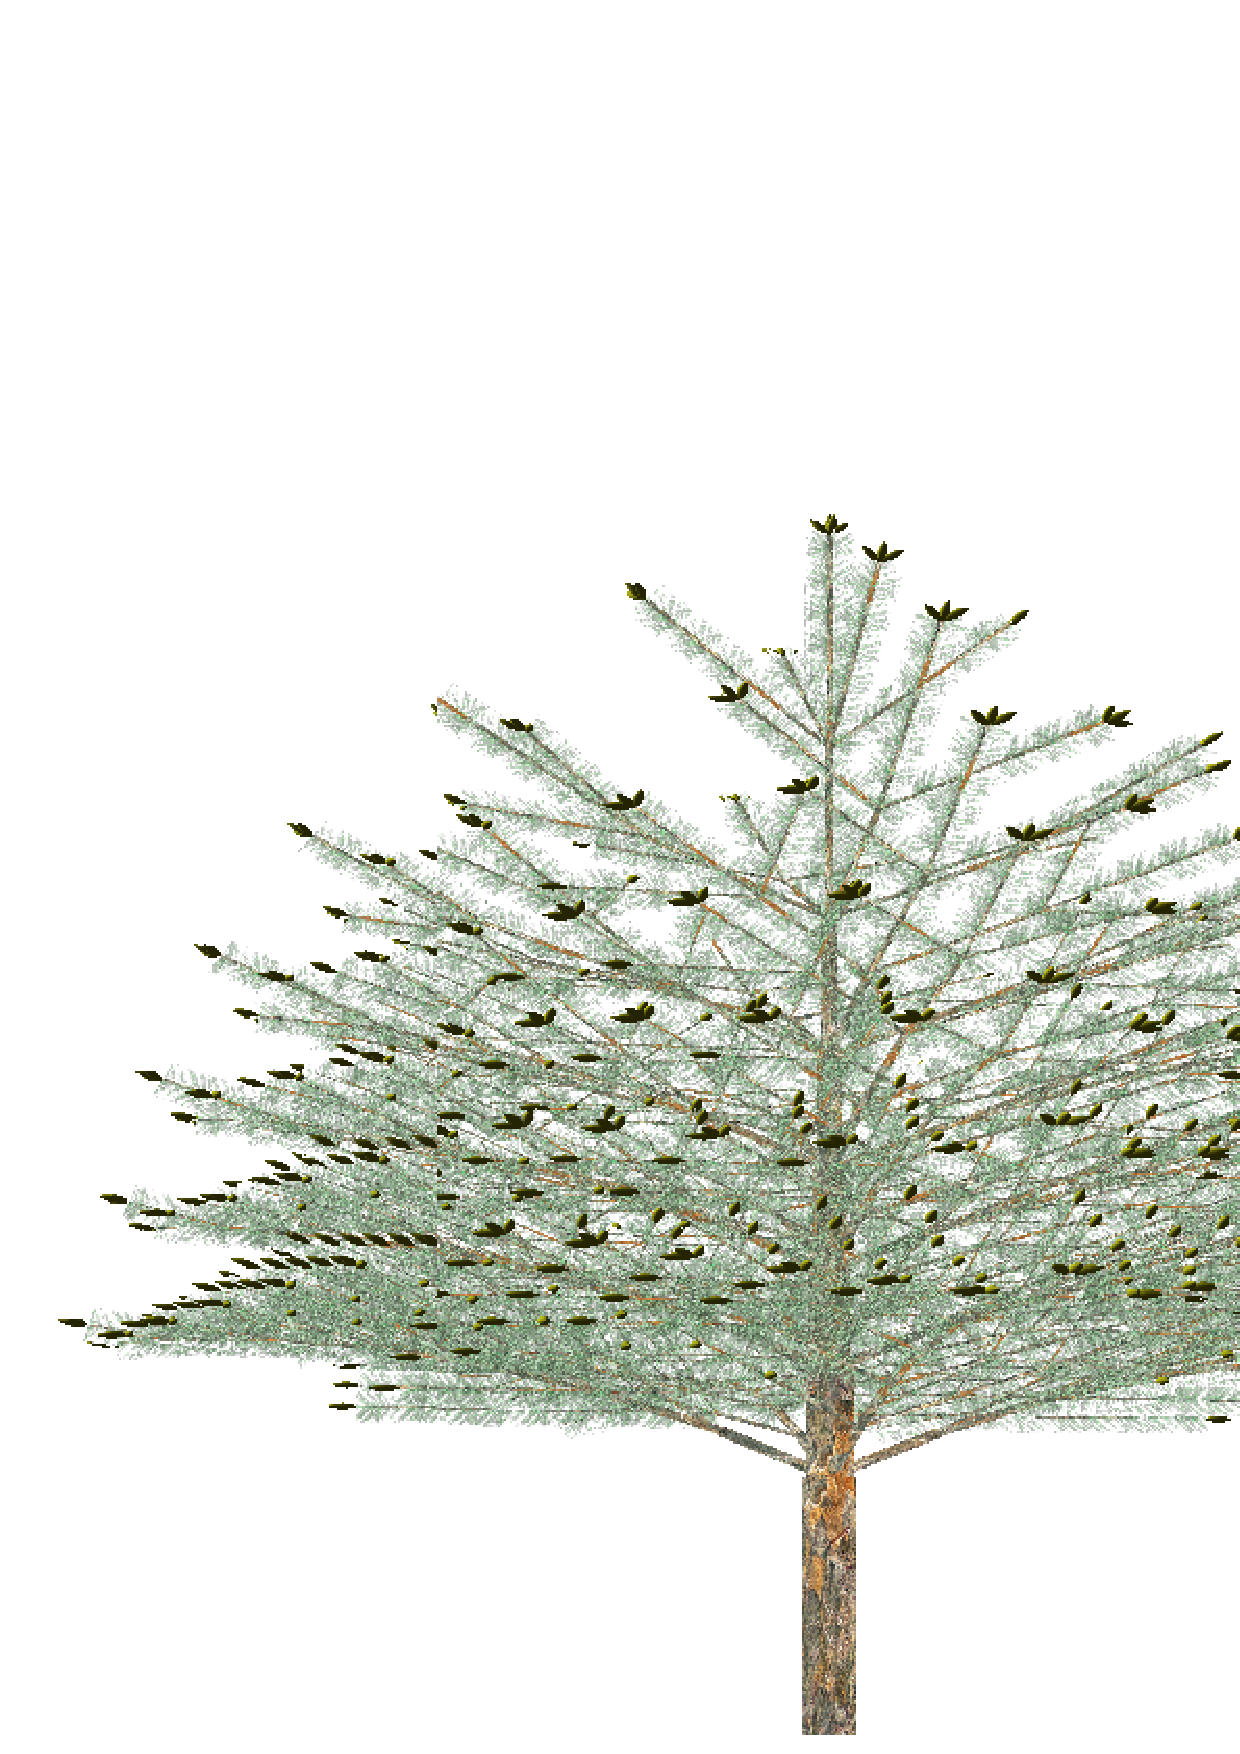
\includegraphics[scale=0.20]{pine8FEM98}
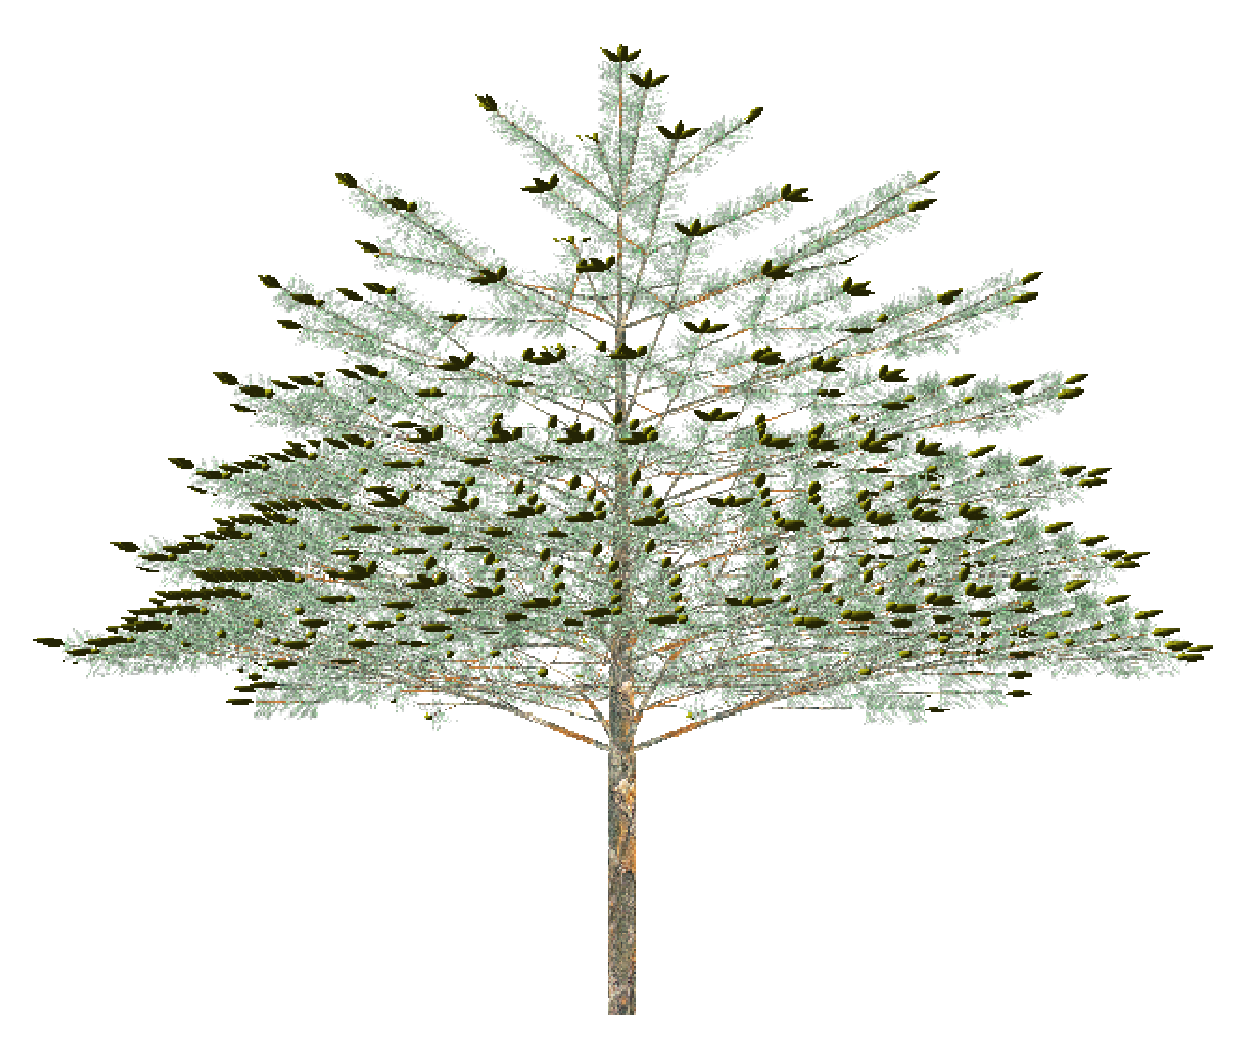
\includegraphics[scale=0.20]{pine8F1}   \caption{The   development  of
  three  pines  after   eight  development  steps  when  architectural
  development  takes place  according  to the  L  program of  Appendix
  \ref{sec:L1} and metabolic functioning is as in \citet{perttunen:96,
    perttunen:98}.  Leftmost:  Development according to  the L program
  only;  middle  and  right:  interaction  of L  language  and  LIGNUM
  depicting the effect of  foliage mortality.  Middle: Foliage remains
  for 5  years.  Length  = 3.5 m,  diameter at  base = 10  cm.  Right:
  Foliage remains for 1 year.  Length = 2.7 m, diameter at base 6 cm.}
\label{fig:pine} \end{figure}

